% =========================================================
% PART V -- MODEL ESTIMATION
% =========================================================

\section{Model Estimation}

% ---------------------------------------------------------
% 32. PARAMETRIC MODEL ESTIMATION
% ---------------------------------------------------------

\begin{frame}{32. Parametric Model Estimation}

\textbf{Definition}

Parametric model estimation assumes that the population
distribution belongs to a known family of distributions
described by a finite number of parameters.

\textbf{Examples}

\begin{itemize}
    \item Normal distribution -- parameters $\mu$ and $\sigma^2$
    \item Bernoulli distribution -- parameter $p$
    \item Poisson distribution -- parameter $\lambda$
\end{itemize}

\vspace{0.1cm}

A parametric model can be written as
\[
\boxed{
f(x;\theta)
}
\]

where $\theta$ represents the unknown parameter(s).

\textbf{Goal}

Estimate the unknown parameters using observed sample data.

\end{frame}


% ---------------------------------------------------------
% 32.1 PARAMETRIC MODEL -- EXAMPLE
% ---------------------------------------------------------

\begin{frame}{32.1 Parametric Model Estimation -- Example}

\textbf{Example}

Suppose a population is assumed to follow a normal distribution:
\[
X\sim N(\mu,\sigma^2)
\]

The parameters are:
\[
\mu=\text{population mean}
\]
\[
\sigma^2=\text{population variance}
\]

Given a sample, we can estimate these parameters using:
\[
\hat{\mu}=\bar{x}
\]

\[
\hat{\sigma}^2=s^2
\]

The assumed distribution provides a mathematical model, while
the sample data is used to estimate its unknown parameters.

\end{frame}


% ---------------------------------------------------------
% 33. MAXIMUM LIKELIHOOD ESTIMATION
% ---------------------------------------------------------

\begin{frame}{33. Maximum Likelihood Estimation}

\textbf{Definition}

Maximum Likelihood Estimation (MLE) is a method for estimating
unknown parameters by choosing the parameter values that make
the observed data most likely.

For observations
\[
x_1,x_2,\ldots,x_n
\]

the likelihood function is
\[
\boxed{
L(\theta)
=
\prod_{i=1}^{n}f(x_i;\theta)
}
\]

The maximum likelihood estimator is
\[
\boxed{
\hat{\theta}
=
\arg\max_{\theta}L(\theta)
}
\]

Choose the parameter value that gives the highest likelihood
for the observed data.

\end{frame}


% ---------------------------------------------------------
% 33.1 MLE -- LOG-LIKELIHOOD
% ---------------------------------------------------------

\begin{frame}{33.1 Maximum Likelihood Estimation -- Log-Likelihood}

Since likelihoods involve products, it is often easier to
maximize the logarithm of the likelihood.

The log-likelihood is
\[
\boxed{
\ell(\theta)=\log L(\theta)
}
\]

Therefore,
\[
\boxed{
\hat{\theta}
=
\arg\max_{\theta}\ell(\theta)
}
\]

Because the logarithm is a monotonically increasing function,
\[
\arg\max_{\theta}L(\theta)
=
\arg\max_{\theta}\log L(\theta)
\]

\textbf{Advantage}

The logarithm converts products into sums, making
mathematical calculations easier.

\end{frame}


% ---------------------------------------------------------
% 33.2 MLE -- SIMPLE EXAMPLE
% ---------------------------------------------------------

\begin{frame}{33.2 Maximum Likelihood Estimation -- Example}

\textbf{Example: Bernoulli Distribution}

Let
\[
X\in\{0,1\}, \qquad P(X=x)=p^x(1-p)^{1-x}
\]

where $p$ is the unknown probability of success.

For observations $x_1,\ldots,x_n$, the likelihood is
\[
L(p)=\prod_{i=1}^{n}p^{x_i}(1-p)^{1-x_i}
\]

The MLE is obtained by maximizing $L(p)$:
\[
\boxed{\hat{p}=\frac{1}{n}\sum_{i=1}^{n}x_i}
\]

$\hat p$ is the \textbf{sample proportion of successes}.

\end{frame}


% ---------------------------------------------------------
% 34. NON-PARAMETRIC MODEL ESTIMATION
% ---------------------------------------------------------

\begin{frame}{34. Non-parametric Model Estimation}

\textbf{Definition}

Non-parametric model estimation does not assume that the
population distribution belongs to a specific parametric family.

Instead, the distribution is estimated directly from the
observed data.

\textbf{Examples}

\begin{itemize}
    \item Empirical Cumulative Distribution Function (ECDF)
    \item Kernel Density Estimation (KDE)
\end{itemize}

\textbf{Key idea}
\[
\boxed{
\text{Data}
\longrightarrow
\text{Estimate Distribution}
}
\]
without requiring a fixed distribution such as normal,
Poisson, or Bernoulli.

\textbf{Advantage}

Flexible when the underlying distribution is unknown or
does not fit a simple parametric family.

\end{frame}


% ---------------------------------------------------------
% 35. EMPIRICAL CDF
% ---------------------------------------------------------

\begin{frame}{35. Empirical CDF}

\textbf{Definition}

The Empirical Cumulative Distribution Function (ECDF) estimates
the cumulative distribution function directly from sample data.

\vspace{0.4cm}

For a sample
\[
x_1,x_2,\ldots,x_n,
\]

the empirical CDF is
\[
\boxed{
F_n(x)
=
\frac{1}{n}
\sum_{i=1}^{n}
\mathbf{1}(x_i\leq x)
}
\]

where $\mathbf{1}(\cdot)$ is the indicator function.

\textbf{Interpretation}

$F_n(x)$ represents the proportion of sample observations
that are less than or equal to $x$.

\end{frame}


% ---------------------------------------------------------
% 35.1 EMPIRICAL CDF -- EXAMPLE
% ---------------------------------------------------------

\begin{frame}{35.1 Empirical CDF -- Example}

Consider the ordered sample:
\[
X=\{10,20,30,40,50\}
\]
Since $n=5$:
\[
F_n(x)
=
\frac{\text{Number of observations}\leq x}{5}
\]

\begin{columns}[T]

\begin{column}{0.48\textwidth}

\[
F_n(30)=0.6
\]

This means that $60\%$ of the observations
are less than or equal to $30$.

\end{column}

\begin{column}{0.48\textwidth}

\begin{table}
\centering
\small

\begin{tabular}{c c}
\toprule
$x$ & $F_n(x)$ \\
\midrule
10 & $1/5=0.2$ \\
20 & $2/5=0.4$ \\
30 & $3/5=0.6$ \\
40 & $4/5=0.8$ \\
50 & $5/5=1.0$ \\
\bottomrule
\end{tabular}

\end{table}

\end{column}

\end{columns}

\end{frame}


% ---------------------------------------------------------
% 36. KERNEL DENSITY ESTIMATION
% ---------------------------------------------------------

\begin{frame}{36. Kernel Density Estimation}

\textbf{Definition}

Kernel Density Estimation (KDE) is a non-parametric method
for estimating the probability density function of a dataset.

\vspace{0.4cm}

For observations $x_1,\ldots,x_n$:

\[
\boxed{
\hat{f}_h(x)
=
\frac{1}{nh}
\sum_{i=1}^{n}
K\left(
\frac{x-x_i}{h}
\right)
}
\]

where:

\begin{itemize}
    \item $K$ = kernel function
    \item $h$ = bandwidth
    \item $n$ = number of observations
\end{itemize}

\end{frame}


% ---------------------------------------------------------
% 36.1 KDE -- BANDWIDTH
% ---------------------------------------------------------

\begin{frame}{36.1 Kernel Density Estimation -- Bandwidth}

The \textbf{bandwidth} $h$ controls the smoothness of the
estimated density.

\textbf{Small bandwidth}

\[
h\downarrow
\quad\Rightarrow\quad
\text{More detailed / less smooth estimate}
\]

\textbf{Large bandwidth}

\[
h\uparrow
\quad\Rightarrow\quad
\text{Smoother estimate}
\]

\textbf{Key idea}

The bandwidth determines how much neighboring observations
influence the estimated density.

\textbf{Application}

KDE is useful for visualizing and estimating unknown
continuous distributions.

\end{frame}


% ---------------------------------------------------------
% 36.2 KDE -- BASIC EXAMPLE
% ---------------------------------------------------------

\begin{frame}{36.2 Kernel Density Estimation -- Example}

\textbf{Example}

Consider the sample:

\[
X=\{2,3,3,4,5\}
\]

KDE places a small smooth kernel around each observation.

\vspace{0.4cm}

The individual kernels are combined to produce an estimated
density:

\[
\boxed{
\text{Individual Kernels}
\longrightarrow
\text{Combined Density Estimate}
}
\]

\vspace{0.4cm}

\textbf{Interpretation}

Instead of assuming that the data follows a normal distribution,
KDE estimates the shape of the distribution directly from the data.

\end{frame}

% ---------------------------------------------------------
% 36.3 KERNEL DENSITY ESTIMATION -- FIGURE
% ---------------------------------------------------------

\begin{frame}{36.3 Kernel Density Estimation -- Figure}

\begin{columns}[T]

\begin{column}{0.62\textwidth}

\centering
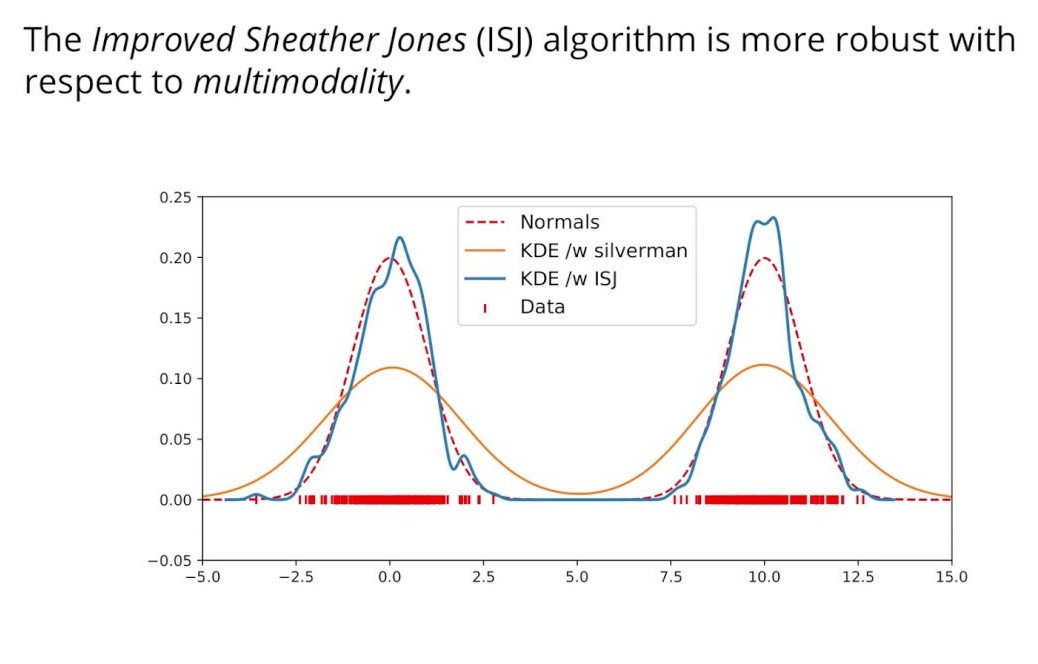
\includegraphics[width=\textwidth]{figures/kde.jpg}

\end{column}

\begin{column}{0.34\textwidth}

\vspace{0.8cm}

The figure shows a smooth density curve
estimated from observed data points.

\vspace{0.4cm}

Unlike a histogram, KDE produces a continuous
estimate of the underlying distribution.

\end{column}

\end{columns}

\end{frame}
% ---------------------------------------------------------
% 37. PARAMETRIC VS NON-PARAMETRIC
% ---------------------------------------------------------

\begin{frame}{37. Parametric vs Non-parametric Model Estimation}

\small

\begin{table}
\centering

\begin{tabular}{>{\bfseries}l l l}
\toprule
Feature & Parametric & Non-parametric \\
\midrule
Distribution assumption &
Specific family &
No fixed family \\

Parameters &
Finite number &
More flexible \\

Flexibility &
Lower &
Higher \\

Examples &
Normal, Poisson &
ECDF, KDE \\

Data requirement &
Often fewer observations &
Often more data needed \\

\bottomrule
\end{tabular}

\end{table}

\vspace{0.4cm}

\textbf{Key idea}

\[
\boxed{
\text{Parametric}
\rightarrow
\text{Assume a distribution}
}
\]

\[
\boxed{
\text{Non-parametric}
\rightarrow
\text{Estimate from data}
}
\]

\end{frame}


% ---------------------------------------------------------
% 37.1 PARAMETRIC VS NON-PARAMETRIC -- APPLICATION
% ---------------------------------------------------------

\begin{frame}{37.1 Parametric vs Non-parametric -- Application}

\textbf{Parametric estimation}

Useful when a suitable probability distribution can reasonably
describe the data.

\vspace{0.1cm}

\textbf{Non-parametric estimation}

Useful when the underlying distribution is unknown,
irregular, or difficult to represent using a simple
parametric model.

\vspace{0.1cm}

\textbf{In AI and Data Science}

The choice depends on:

\begin{itemize}
    \item Amount of available data
    \item Distributional assumptions
    \item Required flexibility
    \item Computational cost
    \item Purpose of the analysis
\end{itemize}

\vspace{0.1cm}

\end{frame}